\documentclass[12pt,oneside,a4paper]{article}

\usepackage[utf8]{inputenc} % Lærer LaTeX at forstå unicode - HUSK at filen skal
% være unicode (UTF-8), standard i Linux, ikke i
% Win.

\usepackage[danish]{babel} % Så der fx står Figur og ikke Figure, Resumé og ikke
% Abstract etc. (god at have).

\usepackage{graphicx}
\usepackage{amsfonts}
\usepackage{amsthm}        % Theorems
\usepackage{amsmath}
%\usepackage{hyperref}

%\renewcommand{\mid}[1]{{\rm E}\!\left[#1\right]}
\newcommand{\bas}{\begin{eqnarray*}}
\newcommand{\eas}{\end{eqnarray*}}
\newcommand{\be}{\begin{equation}}
\newcommand{\ee}{\end{equation}}
\newcommand{\bea}{\begin{eqnarray}}
\newcommand{\eea}{\end{eqnarray}}

\newtheorem{thm}{Sætning}[section]
\newtheorem{mydef}[thm]{Definition}
\newtheorem{eks}[thm]{Eksempel}

\DeclareMathSymbol{,}{\mathord}{letters}{"3B}

\title{Eksponentielle funktioner}

\begin{document}

\maketitle

\section{Indledning}
I denne bog kommer vi til at møde mange forskellige funktioner. Vi har allerede
arbejdet med lineære funktioner. I dette kapitel er emnet eksponentielle
funktioner, og i de næste kapitler vil vi møde bl.a. logaritmefunktioner og
potensfunktioner.

Fælles for alle disse funktioner er, at de har en lang række forskellige
anvendelser. Således optræder eksponentielle funktioner bl.a inden for økonomi
(rente og rentes rente), biologi (vækst af bakterier og andre organismer),
fysik (radioaktivitet), m.m.

\section{Renteformlen}
\begin{figure}[ht]
    \centering
    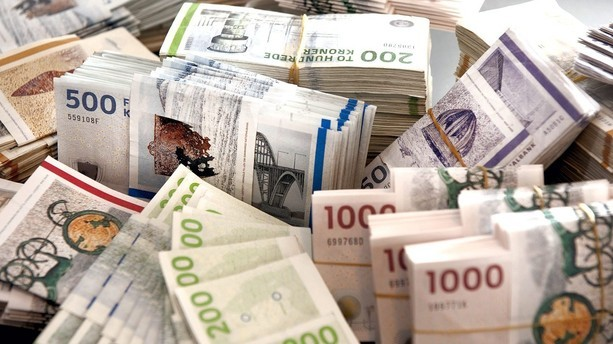
\includegraphics[width=10cm]{penge}
\end{figure}

Vi begynder med et eksempel. Vi har en opsparing på 1000 kroner som vi
indsætter på en opsparingskonto i banken, der giver 5 \% i rente om året. Dvs
efter 1 år bliver der indsat 5 \% af 1000 kroner på kontoen. Det
udregner vi til $ \frac{5}{100} \cdot 1000 = 50 $ kroner. Så efter 1 år står
der nu 1050 kroner på kontoen.  Efter det andet år bliver der nu indsat 5 \% af
1050 kroner, dvs $ \frac{5}{100} \cdot 1050 = 52,50$ kroner.
Det giver et samlet beløb efter 2 år på 1102,50 kroner. Læg mærke til, at rentebeløbet
det andet år (52,50 kroner) er større end rentebeløbet det første år (50 kroner).

Hvis jeg gerne vil beregne, hvad saldoen bliver efter 8 år, så kan man fortsætte ovenstående
beregninger. Det er praktisk at opstille beregningerne i et skema som vist her:
$$
\begin{array}{r|c|l}
    \mbox{efter år} & \mbox{saldo} & \mbox{rentebeløb} \\
    \hline
0 & 1000 & 0,05\cdot 1000 = 50 \\
    \hline
1 & 1050 & 0,05\cdot 1050 = 52,50 \\
    \hline
2 & 1102,50 & 0,05\cdot 1102,50 = 55,13 \\
    \hline
3 & 1157,63 & 0,05\cdot 1157,63 = 57,88 \\
    \hline
4 & 1215,51 & 0,05\cdot 1215,51 = 60,78 \\
    \hline
5 & 1276,29 & 0,05\cdot 1276,29 = 63,81 \\
    \hline
6 & 1340,10 & 0,05\cdot 1340,10 = 67,01 \\
    \hline
7 & 1407,11 & 0,05\cdot 1407,11 = 70,36 \\
    \hline
8 & 1477,47 & 
\end{array}
$$
Det vil sige, at efter 8 år, så vil der stå 1477,47 kroner på saldoen.
Dette er en temmelig besværlig metode, og der er en meget nemmere måde at nå frem til
resultatet 1477,47 kroner på, som vi skal se i det følgende.

For hvert år der går bliver saldoen ganget med
1,05. Dette kan vi indse ved følgende udregning: Efter det første år bliver
saldoen udregnet som: $1050 = 1000 + 50 = 1000 + 0,05\cdot 1000 = 1,05 \cdot 1000$.

Saldoen efter 2 år kan så udregnes som $1,05\cdot 1050 = 1,05 \cdot (1,05 \cdot
1000) = 1,05^2 \cdot 1000$. Saldoen efter 3 år kan på samme måde udregnes som
$1,05\cdot1,05\cdot1,05\cdot 1000 = 1,05^3 \cdot 1000$. Efter 8 år er saldoen
derfor på $1,05^8\cdot 1000$.

Denne metode kan udtrykkes ved følgende formel:
\begin{thm}
    {\em Renteformlen} kan udregne saldoen på en opsparing som begynder med
    værdien $K_0$ og som efter hver {\em termin} bliver forøget med en fast
    rente. Saldoen efter $n$ terminer er givet ved følgende formel:
    $$
    K_n = K_0 \cdot (1+r)^n
    $$
    hvor $K_0$ er {\em startkapitalen}, $r$ er {\em vækstraten}, $n$ er antallet af
    terminer, og $K_n$ er {\em slutkapitalen} efter de $n$ terminer.
\end{thm}
En termin er typisk 1 år, men kan også være f.eks. en måned. Den er bestemt af,
hvor tit der indsættes et nyt rentebeløb. Vækstraten $r$ er renten udtrykt som
decimaltal. Dvs. hvis renten er 5\%, så er vækstraten $r=\frac{5}{100}=0,05$.

I det følgende gennemgår vi nogle eksempler på anvendelse af renteformlen.
\begin{eks}
    Jeg arver 20000 kroner og indsætter beløbet på en
    opsparingskonto som giver 4\% i rente om året. Efter 7 år, hvad vil der stå
    på kontoen?
\end{eks}
\begin{proof}[Svar]
    Først udregnes vækstraten $r=\frac{4}{100} = 0,04$. Så indsættes i renteformlen:
    $$
    K = 20000 \cdot (1 + 0,04)^7 = 26318,64
    $$
    Dvs efter syv år står der lidt over 26000 kroner på saldoen.
\end{proof}

Renteformlen kan også bruges, når man låner penge, hvis man ikke betaler af
(afdrager) på gælden undervejs.
\begin{eks}
    Hvis jeg har en kassekredit med et underskud på 17000 kroner, hvortil der
    lægges 1,8 \% i rente hver måned, hvor meget skylder jeg efter 2 år?
\end{eks}
\begin{proof}[Svar]
    Når rente bliver tilskrevet hver måned, så skal tiden på 2 år omregnes til
    måneder, dvs 24 måneder. Dette er antallet af terminer. Vækstraten er $r =
    \frac{1,8}{100} = 0,018$, og renteformlen giver derfor:
    $$
    K = 17000 \cdot (1 + 0,018)^{24} = 26085,29
    $$
    Den samlede gæld er derfor vokset til over 26000 kroner på de 2 år.
\end{proof}

\section{Eksponentielle funktioner}
Renteformlen er et eksempel på en eksponentiel funktion. I det følgende gennemgår vi en mere generel formel for eksponentielle funktioner, som kan bruges i mange andre sammenhænge end økonomi.

\subsection{Forskrift}
\begin{mydef}
    En eksponentiel funktion er givet ved følgende forskrift:
    $$
    f(x) = b\cdot a^x
    $$
    hvor $a$ kaldes {\em fremskrivningsfaktor},  mens $b$ kaldes {\em
    begyndelsesværdi}. Både $a$ og $b$ vil altid være positive konstanter.
    Definitionsmængden for en eksponentiel funktion er alle tal, dvs $x$ kan
    være både positiv og negativ; værdimængden er alle positive tal, dvs
    $f(x)$ vil altid være positiv.
\end{mydef}


Der er følgende sammenhæng mellem vækstraten $r$ og fremskrivningsfaktoren $a$:
$$
a = 1 + r
$$

\subsection{Grafens udseende}
Eksponentielle funktioner er alle monotone; deres monotoniforhold er bestemt af
fremskrivningsfaktoren: Hvis $a>1$ så er funktionen voksende, hvis $a<1$ så er
funktionen aftagende.
\begin{figure}[ht]
    \centering
    \includegraphics{eksp-b}
    \label{eksp-b}
\end{figure}
På figuren ses to eksempler, én som er voksende (hvor $a=1,4$) og én som er
aftagende (hvor $a=0,9$).

\begin{thm}
    En eksponentiel funktion vil altid skære $y$-aksen i punktet $(0,b)$.
\end{thm}
\begin{proof}
    Dette ses ved at indsætte $x$-koordinaten $x=0$ i forskriften:
    $f(0) = b\cdot a^0 = b\cdot 1 = b$.
\end{proof}

\subsection{Sproglig formulering}
Eksponentielle funktioner optræder hver gang en størrelse vokser eller falder
med en fast procent.

Det er vigtigt at kunne "oversætte" mellem en sproglig beskrivelse og en matematisk beskrivelse.
I det følgende ser vi på nogle eksempler.

\begin{eks}
    Antallet af ænder i et område er på et tidspunkt målt til 270 ænder. Hvert
    år vokser antallet af ænder med 7 \%. Opskriv en eksponentiel funktion.
\end{eks}
\begin{proof}{Svar}
    Dette kan oversættes til følgende formel for antallet af ænder efter $x$ år:
    $$
    f(x) = 270 \cdot 1,07^x
    $$
    Læg mærke til, at fremskrivningsfaktoren er udregnet som $1+\frac{7}{100} =
    1+0,07 = 1,07$.
\end{proof}

\begin{eks}
    Radioaktiviteten af en mængde stof er på et tidspunkt målt til 700. Efter
    hver time falder strålingen med 3\%. Opskriv en eksponentiel funktion.
\end{eks}
\begin{proof}{Svar}
    Radioaktiviteten efter $x$ timer kan udregnes ved følgende forskrift:
    $$
    f(x) = 700 \cdot 0,97^x
    $$
    Her er fremskrivningsfaktoren udregnet som $1 + \frac{-3}{100} = 1-0,03 = 0,97$.
\end{proof}

Man skal også kunne oversætte tilbage, dvs fortolke en forskrift. Vi ser på et eksempel:

\begin{eks}
    Antallet af profiler på et nyt socialt medie er givet ved forskriften
    $$
    f(x) = 10000 \cdot 1,27^x
    $$
    hvor $x$ måles i år. Hvad fortæller tallene i forskriften om antallet af profiler?
\end{eks}
\begin{proof}[Svar]
    Til at begynde med er der 10000 profiler på det nye sociale medie. Hvert år bliver der 27 \% flere profiler.
\end{proof}

\section{Regression}
Eksponentielle funktoner bruges også, når man kun har givet nogle få
data-punkter. Et eksempel kunne være det årlige antal af tvangsopløste
selskaber for en række år, givet ved nedenstående tabel:
$$
\begin{array}{l|c|c|c|c}
    \mbox{År efter 2006} & 0 & 1 & 2 & 3 \\
    \hline
    \mbox{Antal} & 2180 & 2955 & 3698 & 5530
\end{array}
$$
Tabellen skal læses således, at der f.eks. i år 2009 (3 år efter 2006) blev
opløst i alt 5530 selskaber.

Hvis vi indtegner disse fire punkter i et koordinatsystem, så ser vi en tydelig
voksende tendens. Måske kan dette beskrives ved en eksponentiel funktion?

\begin{figure}[ht]
    \centering
    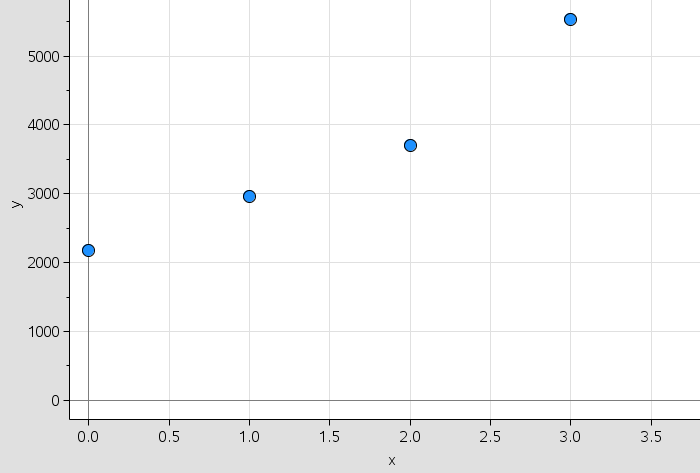
\includegraphics[width=10cm]{eksp-eks1}
\end{figure}

Vi spørger altså, om der findes værdier for tallene $a$ og $b$ som passer med disse punkter. Det viser sig, at overensstemmelsen ikke er perfekt, men at man med {\em regression} kan finde de værdier som passer bedst.

På et CAS-værktøj kan man ved hjælp af eksponentiel regression beregne, at tallene $a$ og $b$ skal have værdierne: 
$$
a = 1,35214
$$
$$
b = 2154,74
$$
Det svarer således til funktionen 
$$
f(x) = 2154,74 \cdot 1,35214 ^x
$$
Tallene i denne forskrift skal fortolkes på følgende måde: I år 2006 var der ca. 2155 tvangsopløste selskaber, og antallet er siden da vokset med ca. 35 \% om året.

Vi kan også tegne grafen for denne eksponentielle funktion og se, at den
passer rimeligt godt med punkterne.

Vi siger her, at den eksponentielle funktion er en {\em model} for antallet af
tvangsopløste selskaber. Den gør os i stand til at {\em forudsige}, hvordan
udviklingen vil fortsætte.

\begin{eks}
    Hvor mange tvangsopløste selskaber vil der være i år 2011?
\end{eks}
\begin{proof}[Svar]
    År 2011 svarer til $x=5$ (5 år efter 2006). Vi udregner:
    $$
    f(5) = 2154,74 \cdot 1,35214^5 = 9738,7
    $$
    Dette resultat fortolker vi som, at den den eksponentielle
    model forudsiger, at ca. 9740 selskaber vil blive tvangsopløst i 2011.
\end{proof}
    

\section{Eksponentialfunktion fastlagt ved to punkter}
Hvis man kun kender to punkter, så vil der være netop én eksponentiel funktion
som går præcist gennem de to punkter. Dette fremgår af følgende sætning:

\begin{thm}
    Hvis en eksponentiel funktion går gennem de to punkter $(x_1, y_1)$ og $(x_2, y_2)$,
    så er tallene $a$ og $b$ givet ved:
    $$
    a = \left(\frac{y_2}{y_1}\right)^{\frac{1}{x_2-x_1}}
    $$
    og
    $$
    b = \frac{y_1}{a^{x_1}}
    $$
\end{thm}
\begin{proof}
    At funktionen går gennem punktet $(x_1, y_1)$ betyder, at $y_1 = f(x_1)$ og tilsvarende for punktet
    $(x_2,y_2)$. Ved at indsætte den generelle forskrift for en eksponentiel funktion, så giver det:
    $$
    y_1 = b\cdot a^{x_1}
    $$
    og 
    $$
    y_2 = b \cdot a^{x_2}
    $$
    Dette er to ligninger med de to ubekendte $a$ og $b$. For at løse denne ligning, så er det smart først
    at isolere $b$ i den første ligning. Det giver:
    $$
    b = \frac{y_1}{a^{x_1}}
    $$
    Dette indsættes i den anden ligning, og så omskrives resultatet:
    \bas
    y_2 &=& \frac{y_1}{a^{x_1}} \cdot a^{x_2} \\
    &=& \frac{y_1 \cdot a^{x_2}}{a^{x_1}} \\
    &=& y_1 \cdot \frac{a^{x_2}}{a^{x_1}} \\
    &=& y_1 \cdot a^{x_2-x_1}
    \eas
    Nu kan vi dividere med $y_1$:
    $$
    \frac{y_2}{y_1} = a^{x_2-x_1}
    $$
    Og til sidst opløfter vi begge sider i potensen $\frac{1}{x_2-x_1}$:
    $$
    \left(\frac{y_2}{y_1}\right)^{\frac{1}{x_2-x_1}} = a
    $$
\end{proof}

Eksempler, hvor man ikke skal bruge denne sætning.
\end{document}

